\documentclass[oneside,senior,etd]{BYUPhysForDegree}

\usepackage[utf8]{inputenc}
\usepackage{rotating} 

\usepackage[russian]{babel}
\usepackage{amsfonts} % Пакеты для математических символов и теорем
\usepackage{amstext}
\usepackage{amssymb}
\usepackage{amsthm}
\usepackage{graphicx} % Пакеты для вставки графики
\usepackage{subfig}
\usepackage{color}
\usepackage[unicode]{hyperref}
\usepackage[nottoc]{tocbibind} % Для того, чтобы список литературы отображался в оглавлении
\usepackage{algorithmic} % Для записи алгоритмов в псевдокоде
\usepackage{algorithm}
\usepackage{verbatim} % Для вставок заранее подготовленного текста в режиме as-is
\usepackage{listings}

\usepackage{diagbox}

\usepackage{commath}
\newcommand\Tau{\mathcal{T}}
\newcommand{\R}{\mathbb{R}}
\usepackage{color}
\usepackage[colorinlistoftodos, prependcaption]{todonotes}
\usepackage{multirow}
\newcommand*{\MyIndent}{\hspace*{0.2cm}}%


\Chair{Кафедра системного программирования}
\Lab{~}
\Year{2024}
  \Month{Февраль}
  \City{Москва}
  \AuthorText{Автор}
  \Author{Морозов Илья Федорович}
  \AuthorEng{Morozov Ilia Fedorovich}
  \AcadGroup{328}
  \TitleTop{Отчёт №1}
  % \TitleTop{JavaPrac}
  % \TitleBottom{с помощью языковых моделей}
  %\TitleMiddle{}
  % \docname{Отчёт № 1}
  
%%%% DON'T change this. It is here because .sty does not support cyrillic cp properly %%%%
\University{Московский государственный университет имени М.В.Ломоносова}
\Faculty{Факультет вычислительной математики и кибернетики}
\GrText{гр. 328}

% КОНЕЦ ТИТУЛЬНОГО ЛИСТА

\begin{document}
\fixmargins
\makepreliminarypages
\oneandhalfspace

\newpage 
 
\newpage
\section{Описание страниц}

При входе страница с кнопкой <<Вход>>. При нажатии на нее всплывает форма с двумя полями: почта, пароль, и кнопкой <<Войти>>. При успешной авторизации происходит переход на страницу с операциями (/operations), где в header есть ссылка для перехода на /operations, а ниже перечень услуг-ссылок, ведущих на соответствующую страницу:
\begin{enumerate}
    \item Списки клиентов:
    
    Поле-фильтр по услугам (по умолчанию -- любая), при нажатии список со всеми услугами из базы данных, затем два поля -- начала и конца временного интервала, по которым хотим фильтровать (предполагают текстовый ввод), последнее поле -- фильтр по наличию задолженности (переключатель "Да" или "Нет"). Рядом кнопка "Поиск", по нажатию на которую выводится выборка из базы данных, где каждая запись удовлетворяет условиям выше и несёт в себе следующую информацию: ФИО, название оказываемой услуги, её сроки.
    
    \item История операций по счетам:
    
    Поле с ФИО клиента(текстовый ввод), далее два поля -- начала и конца временного интервала по которым хотим фильтровать. Рядом кнопка <<Поиск>>, по нажатию на которую выводится выборка из базы данных, где каждая запись удовлетворяет условиям выше и несёт в себе следующую информацию: 
    ФИО, дата начисления/списания, сумма (положительная означает пополнения в рублях, а отрицательная -- списания)
    \item Регистрация договоров об оказании услуг:
    
    Поле -- название услуги, поле -- номер договора, поле -- ФИО клиента. Рядом кнопка <<Добавить>>, по нажатию на которую происходит занесение в базу.
    \item Регистрация поступлений/списаний:
    
    Поле -- ФИО клиента, поле -- сумма, может быть как отрицательной, так и положительной. Рядом кнопка <<Добавить>>, по нажатию на которую происходит занесение в базу.
\newpage
    \item Управление клиентами:
    
    Поле -- ФИО клиента, поле -- название организации, к которой он относится (пусто, если физ. лицо), поле -- моб. телефон, поле -- почта, поле -- адрес. Рядом 4 кнопки <<Найти>>, <<Удалить>> (предполагают заполнение только ФИО, остальные не учитываются), <<Редактировать>>, <<Добавить>> (требует заполнения всех полей). При нажатии <<Найти>>, <<Удалить>> происходит соответствующее действие в базе. При нажатии <<Редактировать>> происходит поиск данного клиента и дальнейшее изменение его данных на проставленные в форме. <<Найти>> работает как описано выше.
    \item Управление услугами:
    
    Поля: название услуги, кол-во минут в услуге, кол-во смс, кол-во интернета в Мбайт, максимальное число пользователей, цена услуги, цена минуты при исчерпании пакета, цена смс при исчерпании пакета, цена мобильного интернета за Мбайт при исчерпании пакета. Кнопки полностью аналогичны кнопкой <<Управление клиентами>>.
\end{enumerate}

С каждой из этой страниц есть переход к общему перечню операций (/operations) по ссылке в header.

\newpage
\section{Сценарии использования}

Пользователь, заходя на сайт, проходит обязательную аутентификацию, посредством нажатия на кнопку <<Вход>>, соответственно. При аутентификации, в случае неверного ввода выводится текст, сигнализирующий об этом. Далее ожидается повторное заполнение формы. В случае верного окно исчезает, и пользователь получает доступ к основному функционалу сайта, а именно попадает на страницу (/operation) со всеми операциями с базой.

В секции №1 описаны какие ссылки имеются на этой странице. При выборе происходит переход на конкретную страницу с полями, которые заполняются пользователем и по нажатию кнопки (например, <<Найти>>, <<Редактировать>>, <<Удалить>>, <<Добавить>>) происходит действие, описанное также в секции №1.

Опишем возможные сценарии: 
\begin{enumerate}
    \item Получение списка клиентов, в т.ч. по оказываемым услугам в заданном интервале времени, по характеристикам их счетов:
    нажатие кнопки <<Вход>> --> заполнение полей с почтой, паролем --> нажатие кнопки <<Войти>> --> клик по ссылке <<Списки клиентов>> --> заполнение(выбор из предложенных вариантов) полей с оказываемой услугой, началом и концом временного интервала, наличием задолженности --> нажатие кнопки <<Найти>>.

    \item Получение росписи операций по счету клиента за заданный интервал времени:
    нажатие кнопки <<Вход>> --> заполнение полей с почтой, паролем --> нажатие кнопки <<Войти>> --> клик по ссылке <<История операций по счетам>> --> заполнение полей с началом и концом временного интервала, ФИО --> нажатие кнопки <<Найти>>.

    \item Регистрация договора об оказании услуги:
    нажатие кнопки <<Вход>> --> заполнение полей с почтой, паролем --> нажатие кнопки <<Войти>> --> клик по ссылке <<Регистрация договоров об оказании услуг>> --> заполнение полей с названием услуги, номером договора, ФИО клиента --> нажатие кнопки <<Добавить>>.

    \item Регистрация поступлений на счет и списаний:
    нажатие кнопки <<Вход>> --> заполнение полей с почтой, паролем --> нажатие кнопки <<Войти>> --> клик по ссылке <<Регистрация поступлений/списаний>> --> заполнение полей с ФИО, суммой (отрицательная -- списание, положительная -- начисление) --> нажатие кнопки <<Добавить>>.

    \item Добавление данных о клиенте:
    нажатие кнопки <<Вход>> --> заполнение полей с почтой, паролем --> нажатие кнопки <<Войти>> --> клик по ссылке <<Управление клиентами>> --> заполнение полей с ФИО, названием организации, к которой он относится (пусто, если физ. лицо), моб. телефон, почта, адрес --> нажатие кнопки <<Добавить>>.

    \item Удаление данных о клиенте:
    нажатие кнопки <<Вход>> --> заполнение полей с почтой, паролем --> нажатие кнопки <<Войти>> --> клик по ссылке <<Управление клиентами>> --> заполнение поля с ФИО --> нажатие кнопки <<Удалить>>.

    \item Чтение данных о клиенте:
    нажатие кнопки <<Вход>> --> заполнение полей с почтой, паролем --> нажатие кнопки <<Войти>> --> клик по ссылке <<Управление клиентами>> --> заполнение поля с ФИО --> нажатие кнопки <<Найти>>.

    \item Редактирование данных о клиенте:
    нажатие кнопки <<Вход>> --> заполнение полей с почтой, паролем --> нажатие кнопки <<Войти>> --> клик по ссылке <<Управление клиентами>> --> заполнение формы с полями ФИО, названием организации, моб. телефоном, почтой, адресом --> нажатие кнопки <<Редактировать>>.

    \item Добавление и удаление услуги, чтение и редактирование данных о ней:
    аналогично пункту выше, только другие поля: название услуги, кол-во минут в услуге, кол-во смс, кол-во интернета в Мбайт, максимальное число пользователей, цена услуги, цена минуты при исчерпании пакета, цена смс при исчерпании пакета, цена мобильного интернета за Мбайт при исчерпании пакета.

\end{enumerate}

\newpage
Таким образом, общая схема навигации по сайту выглядит так:

\begin{figure}[hbt!]
    \centering
    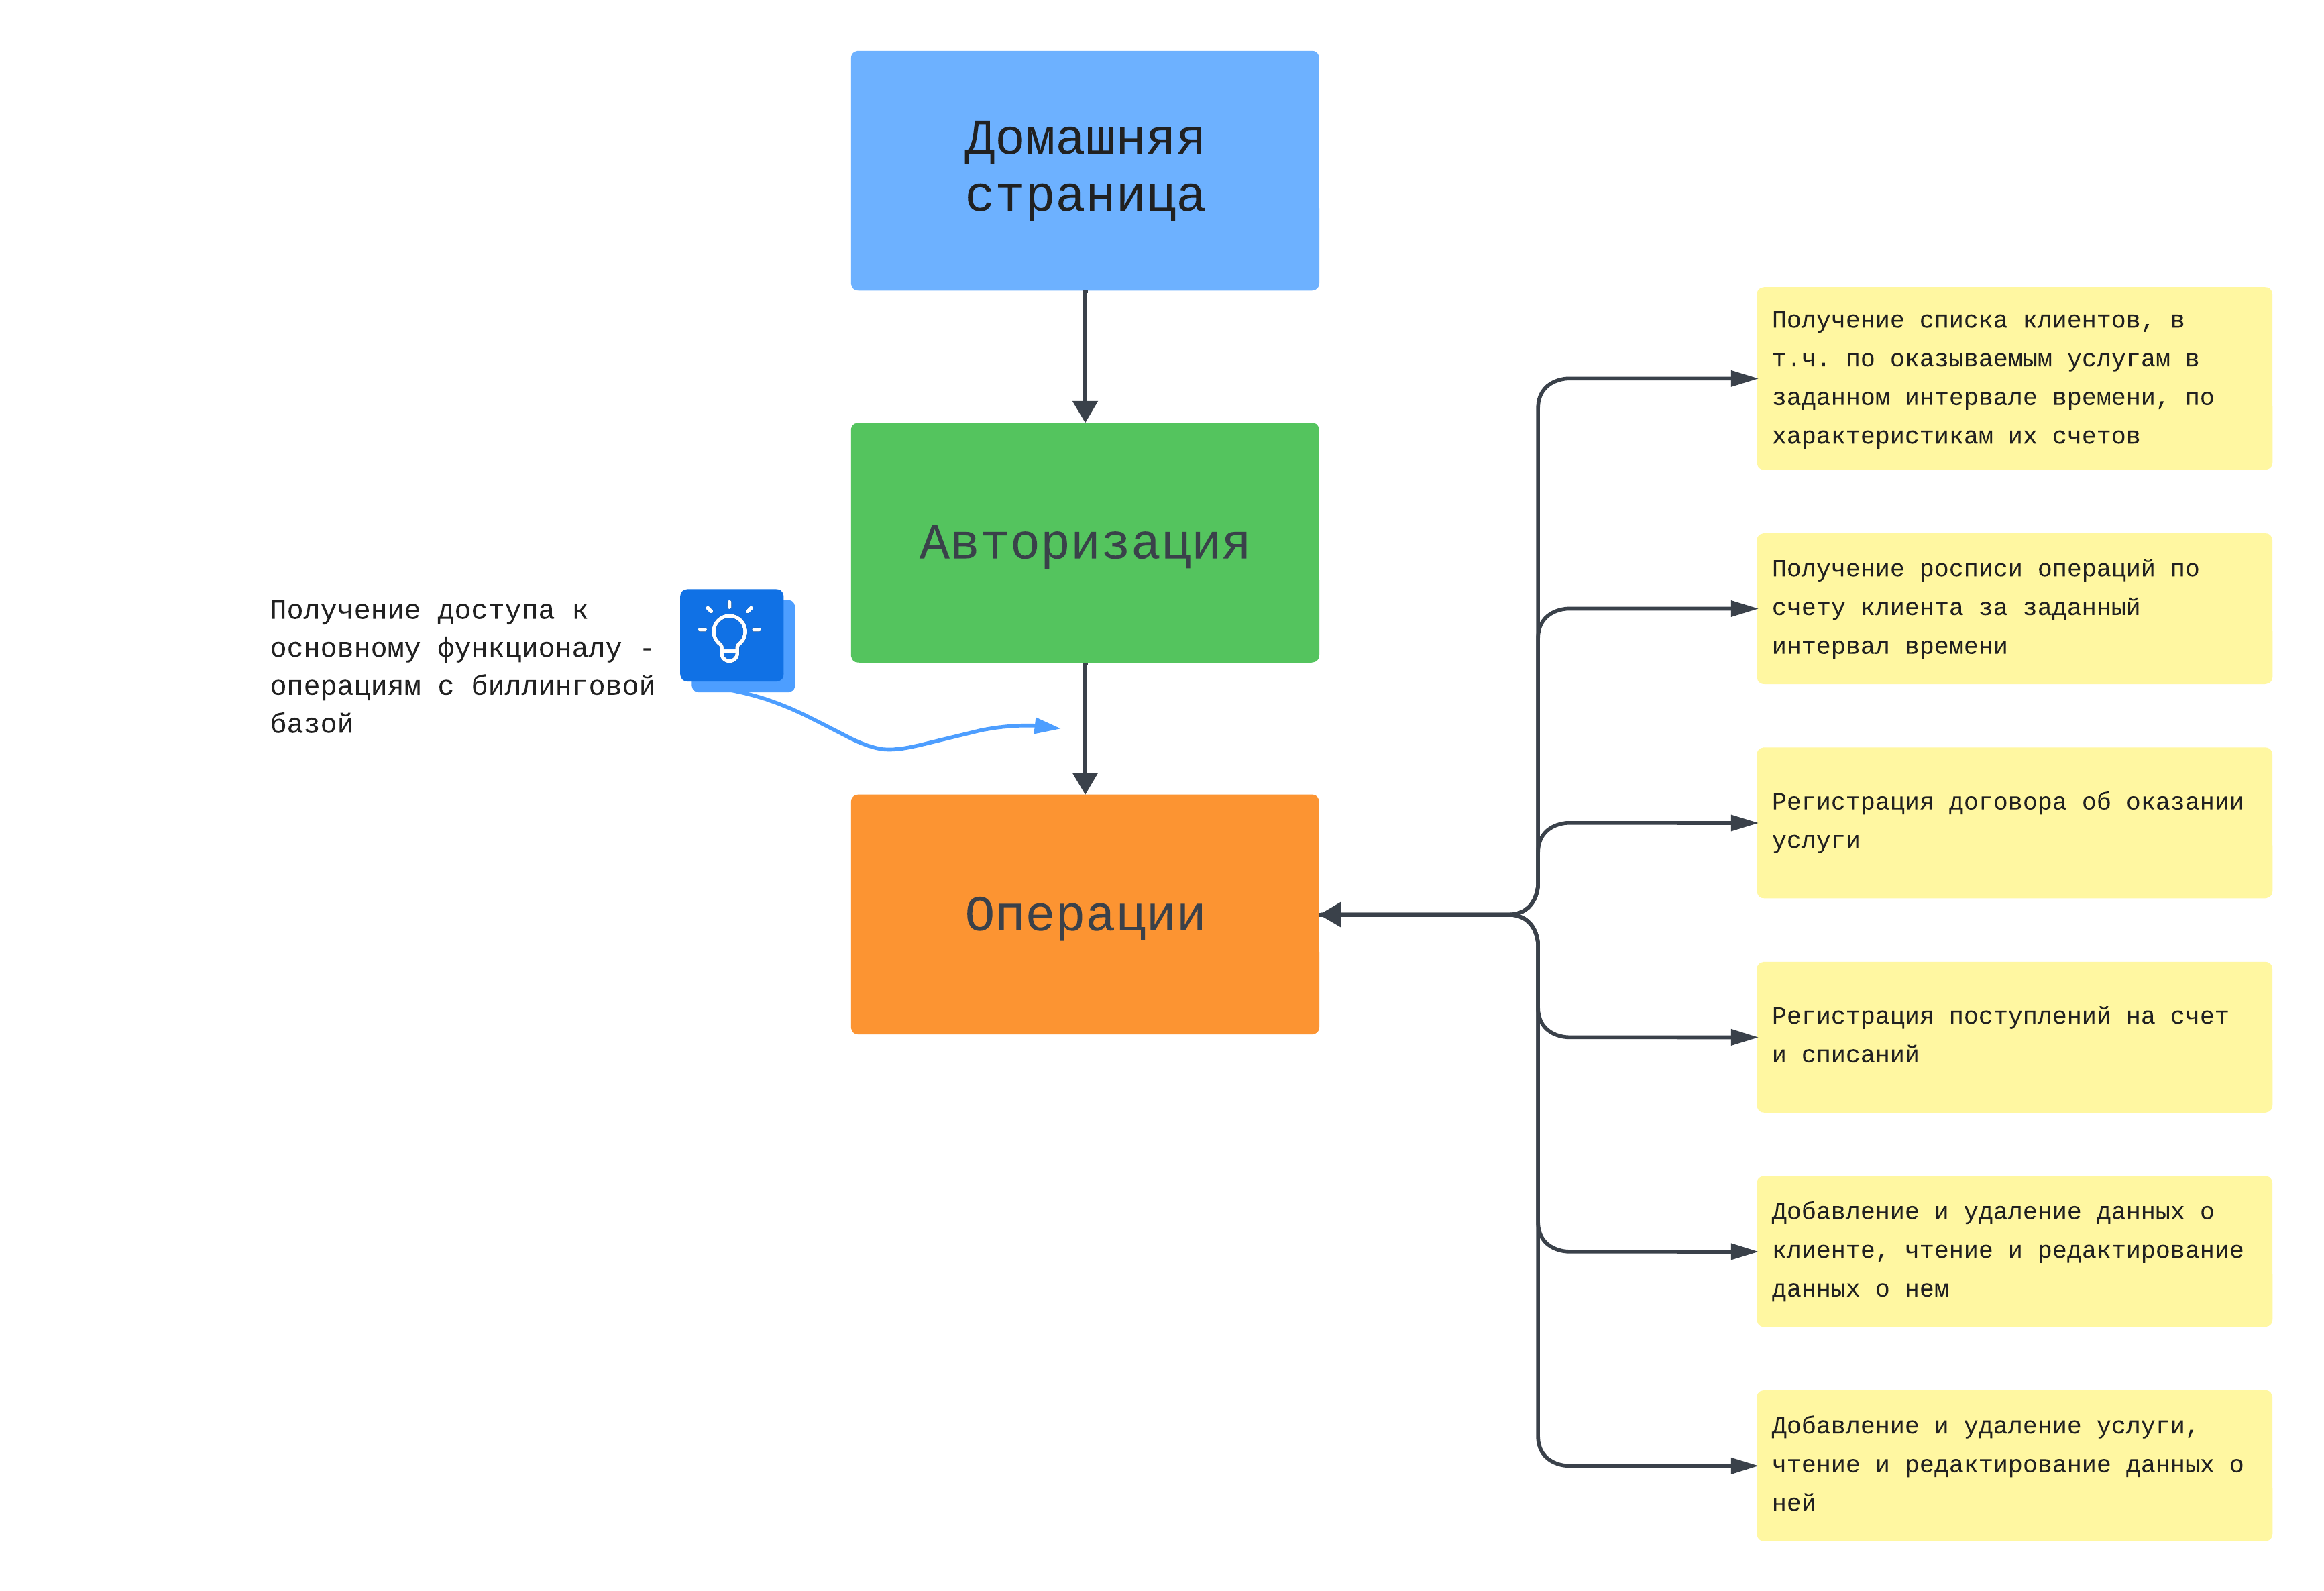
\includegraphics[width=1.0\linewidth]{sitemap.png}
    \caption{Навигация.}
    \label{fig:sitemap}
\end{figure}

\newpage
\section{База данных}

Снизу приведена схема базы данных, которой мы и будем пользоваться. Опишем таблицы и поля, которые в ней есть:
\begin{enumerate}
    \item Услуги: \begin{itemize}
        \item Наименование услуги
        \item Характеристики пакета в формате json:
        
        Кол-во минут "min": число, кол-во смс "sms": число, мобильный интернет в Мбайт "internet": число, максимальное число клиентов в пакете "max\_members": число.
        \item Тарифный план в формате json:
        
        Цена услуги "tariff": число, цена минуты при исчерпании пакета "extra\_min": число, цена смс при исчерпании пакета "extra\_sms": число, цена мобильного интернета за Мбайт при исчерпании пакета  "extra\_internet": число.
    \end{itemize}
    \item Организации, первая запись в этой таблице -- 'Физ. лицо' для дальнейшего удобства: \begin{itemize}
        \item Название организации
        \item ИНН
    \end{itemize}

    \item Счета: \begin{itemize}
        \item Баланс
        \item История поступлений/списаний в формате json:
        
        Массив пар: ключ хранит дату, а значение -- пополнение/списание в рублях (отрицательное число -- списание, положительное -- пополнение)
        \item Размер максимального кредита
        \item Сроки его погашения
    \end{itemize}

    \item Клиенты, здесь под клиентом понимается именно человек, если он является Физ. лицом, то поле "client\_org" будет указывать на первую запись, иначе -- на соответствующую организацию: \begin{itemize}
        \item Ключ на организацию
        \item ФИО клиента
        \item Информация о клиенте в формате json:

        Телефон "phone": строка, почта "email": строка, адрес "address": строка
        \item Ключ на счёт клиента в billing.accounts, реализована связь 1--1.
    \end{itemize}
    \item Таблица <<Client\_Service>> для связи многие-ко-многим, помимо ключей содержит: \begin{itemize}
        \item Номер договора
        \item Начало оказания услуги
        \item Конец оказания услуги, NULL - если еще активно
    \end{itemize}

\end{enumerate}
\begin{figure}[hbt!]
    \centering
    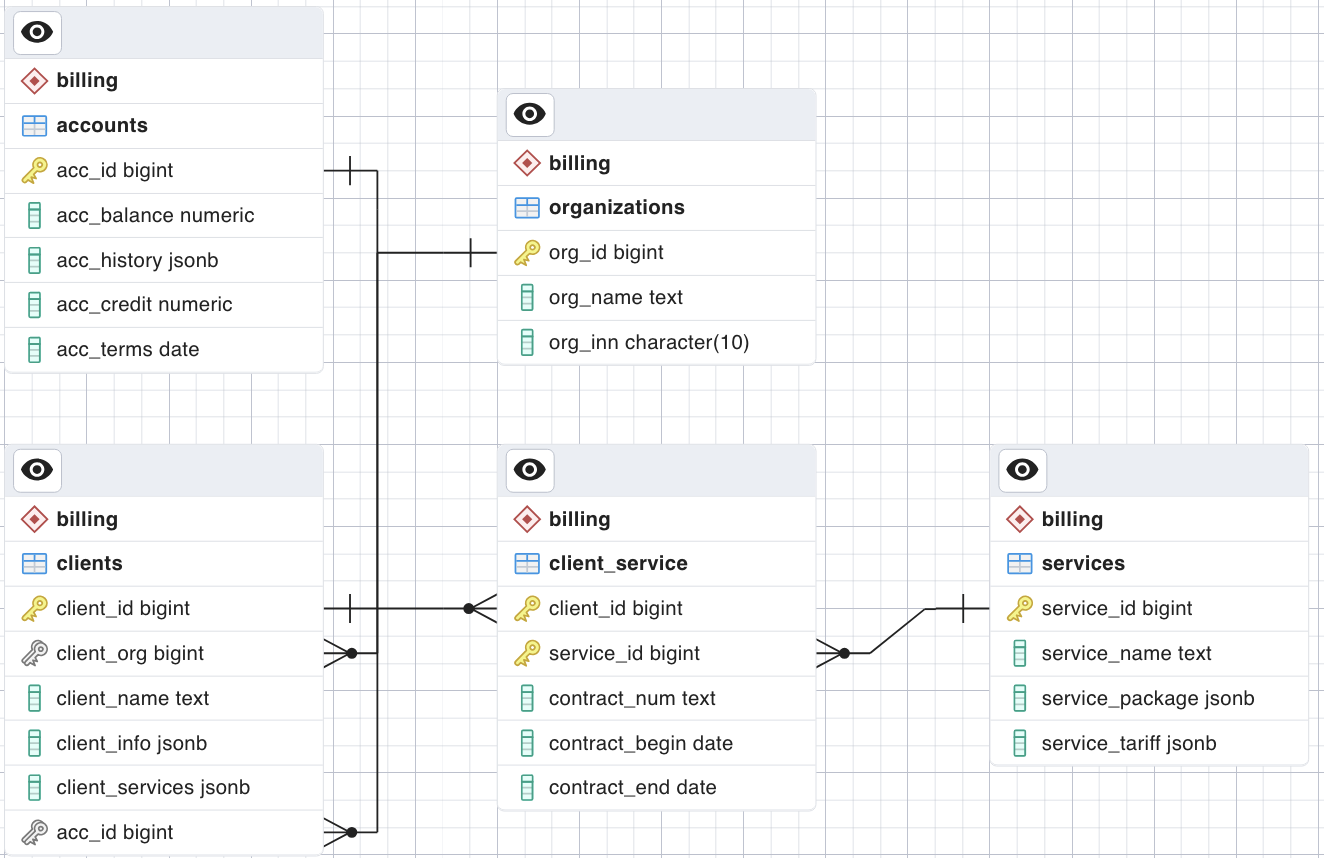
\includegraphics[width=1.0\linewidth]{scheme.png}
    \caption{Схема базы данных.}
    \label{fig:scheme}
\end{figure}



\end{document}